\subsubsection{Beskrivelse}
En kondensator (engelsk: capasitor)
er en av de mest fundamentale kompenentene vi bruker.
Dens funksjon er å lagre elektrisk ladning.
De brukes bl.a. til lokal energilagring (som et lite batteri),
dempe brå forandring av spenning (for å beskytte sårbare komponenter)
og signalfiltrering.



\subsubsection{Virkemåte og symbol}
En kondensator består av to ledende plater
med et isolerende materiale (et dielektrisk) i mellom.
\\
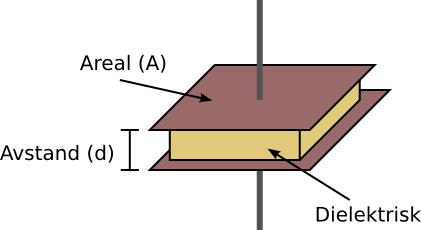
\includegraphics[width=0.5\textwidth]{./img/kondensator-basic}
\\\\
\emph{Symbolet} for en kondensator gjenspeiler oppbygningen.
\\
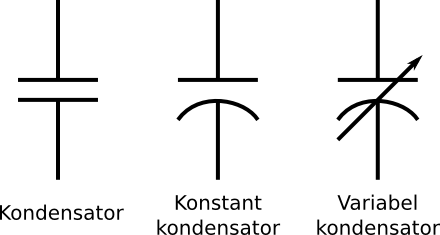
\includegraphics[width=0.5\textwidth]{./img/kondensator-symboler}
\\
\paragraph{Spenning} \mbox{} \\
Når en kondensator kobles til en spenningskilde
vil det gå strøm gjennom kretsen.
Elektronene strømmer \emph{mot} den ene siden av kondensatoren,
og \emph{fra} den andre siden.
\\
Men strømmen blir blokkert av dielektrikumet
og går ikke gjennom kondensatoren.
Istedenfor samler elektronene seg på den ene siden,
og det blir en mangel på elektroner på andre siden.
\\
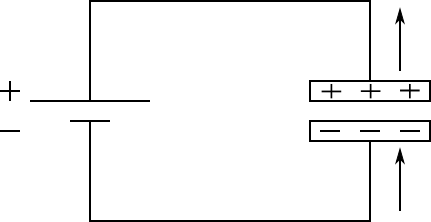
\includegraphics[width=0.5\textwidth]{./img/kondensator-ladning}
\\
Man kan tenke på det som om det går to strømmer.
En fra negativ pol til kondensatoren.
Og en fra kondensatoren mot positiv pol.
\\\\
Nå er det negative ladninger på den ene siden,
og positive på den andre.
Det vil si at vi har en spenning over kondensatoren.



\subsubsection{Formler og enheter}
Kapasitet (C), evnen til å lagre ladning, er gitt ved følgende formel.
$$C = \frac{Q}{V} = \frac{Ladning}{Spenning}$$
Enheten for kapasitet er farad (F).
\\
En 1 farads kondensator ladet med 1 coulomb
har en spenning på 1 volt mellom platene.
\\\\
Kapasiteten til en kondensator er avhengig av
arealet til flatene, avstanden mellom dem og dielektrikumet i mellom.
$$C = \varepsilon _0 \cdot \varepsilon _r \cdot \frac{A}{d}$$
C = kapasitet i farad \\
$\varepsilon _0 =$ permittiviteten til dielektrikumet i vakuum \\
$\varepsilon _r =$ relativ permittivitet til dielektrikumet\\
$A =$ arealet til overflatene til platene \\
$d =$ avstand mellom platene i meter
\\\\
Serie- og parallellkobling fungerer motsatt
av hvordan vi er vant med å tenke med motstander.
Vi ser på en seriekobling \\
\begin{circuitikz} \draw
(0,0) to[C, label=$C_1$] (2,0)
      to[C, label=$C_2$] (4,0)
      to[C, label=$C_3$] (6,0)
      ;
\end{circuitikz} \\
Den totale kapasiteten er gitt ved.
$$\frac{1}{C_T} = \frac{1}{C_1} + \frac{1}{C_2} + \frac{1}{C_3}$$
Tilsvarende for parallellkobling \\
\begin{circuitikz} \draw
(0,0) -- (6,0)
      -- (6,2)
      -- (0,2)
(2,0) to[C, label=$C_1$] (2,2)
(4,0) to[C, label=$C_2$] (4,2)
(6,0) to[C, label=$C_3$] (6,2)
      ;
\end{circuitikz} \\
Den totale kapasiteten er gitt ved.
$$C_T = C_1 + C_2 + C_3$$
